%%%%%%%%%%%%%%%%%%%%%%%%%%%%%%%%%%%%%%%%%%%%%%%%%%%%%%%%%%%%%%%%%%%%%%%%%%%%%%%%%%%%%%%%%%%%%%%%%%%%%%%%%%%%%%%%%%%%%%%%%%%%%%%%%%%%%%%%%%%%%%%%%%%%%%%%%%%%%%%%%%%%%%%%%%%%%%%%%%%%%%%%%%%%
% Written By Michael Brodskiy
% Class: AP Chemistry
% Professor: J. Morgan
%%%%%%%%%%%%%%%%%%%%%%%%%%%%%%%%%%%%%%%%%%%%%%%%%%%%%%%%%%%%%%%%%%%%%%%%%%%%%%%%%%%%%%%%%%%%%%%%%%%%%%%%%%%%%%%%%%%%%%%%%%%%%%%%%%%%%%%%%%%%%%%%%%%%%%%%%%%%%%%%%%%%%%%%%%%%%%%%%%%%%%%%%%%%

\documentclass[12pt]{article} 
\usepackage{alphalph}
\usepackage[utf8]{inputenc}
\usepackage[russian,english]{babel}
\usepackage{titling}
\usepackage{amsmath}
\usepackage{graphicx}
\usepackage{enumitem}
\usepackage{amssymb}
\usepackage[super]{nth}
\usepackage{expl3}
\usepackage[version=4]{mhchem}
\usepackage{hpstatement}
\usepackage{rsphrase}
\usepackage{everysel}
\usepackage{ragged2e}
\usepackage{geometry}
\usepackage{fancyhdr}
\usepackage{cancel}
\usepackage{siunitx}
\usepackage{chemfig}
\geometry{top=1.0in,bottom=1.0in,left=1.0in,right=1.0in}
\newcommand{\subtitle}[1]{%
  \posttitle{%
    \par\end{center}
    \begin{center}\large#1\end{center}
    \vskip0.5em}%

}
\newcommand{\orbital}[2]{{%
    \def\+{\big|\hspace{-2pt}\overline{\underline{\hspace{2pt}\upharpoonleft}}}%
    \def\-{\overline{\underline{\downharpoonright\hspace{2pt}}}\hspace{-2pt}\big|}%
    \def\0{\big|\hspace{-2pt}\overline{\underline{\phantom{\hspace{2pt}\downharpoonright}}}}%
    \def\1{\overline{\underline{\phantom{\downharpoonright\hspace{2pt}}}}\hspace{-2pt}\big|}%
  \setlength\tabcolsep{0pt}% remove extra horizontal space from tabular
  \begin{tabular}{c}$#2$\\[2pt]#1\end{tabular}%
}}
\DeclareSIUnit\Molar{\textsc{m}}
\DeclareSIUnit\atm{\textsc{atm}}
\DeclareSIUnit\torr{\textsc{torr}}
\DeclareSIUnit\psi{\textsc{psi}}
\DeclareSIUnit\bar{\textsc{bar}}
\DeclareSIUnit\Celsius{\textsc{C}}
\usepackage{hyperref}
\hypersetup{
colorlinks=true,
linkcolor=blue,
filecolor=magenta,      
urlcolor=blue,
citecolor=blue,
}

\urlstyle{same}


\title{Chapter 13 $-$ Acid-Base Reactions}
\date{\today}
\author{Michael Brodskiy\\ \small Instructor: Mr. Morgan}

% Mathematical Operations:

% Sum: $$\sum_{n=a}^{b} f(x) $$
% Integral: $$\int_{lower}^{upper} f(x) dx$$
% Limit: $$\lim_{x\to\infty} f(x)$$

\begin{document}

\maketitle

\begin{itemize}

  \item Bronsted-L\o wry acid $-$ donates \ce{H+}, base takes \ce{H+}

  \item Arrhenius $-$ Acids take \ce{OH-}, bases gives off \ce{OH-}

  \item \ce{H3PO4 + C2H3O2 <-> H2PO4- + HC2H3O2+} conjugate acid/base example

    \begin{enumerate}

      \item \ce{H2PO4-} is the conjugate base pair of \ce{H3PO4}, while \ce{HC2H3O2+} is the conjugate acid pair of \ce{C2H3O2}

      \item Conjugate acid/base pairs differ by one \ce{H+} (nothing else)

    \end{enumerate}

  \item Ion Product ($k_w$)

    \begin{enumerate}

      \item For water, $k_w=[\ce{H+}][\ce{OH-}]=1\cdot10^{-14}$

    \end{enumerate}

  \item Acid-Base Determination

    \begin{enumerate}

      \item $[\ce{H+}] > [\ce{OH-}]$ acidic

      \item $[\ce{H+}] < [\ce{OH-}]$ basic

      \item $[\ce{H+}] = [\ce{OH-}]$ neutral

    \end{enumerate}

  \item pH formulas

    \begin{enumerate}

      \item pH=$-\log\left[ \ce{H+} \right]$

      \item pOH=$-\log\left[ \ce{OH-} \right]$

      \item pH + pOH = 14

      \item \begin{tabular}[H]{c c c c c c c}
          acidic & 0 & $\leftrightarrow$ & 7 & $\leftrightarrow$ & 14 & basic
        \end{tabular}

    \end{enumerate}

  \item Logarithms without a calculator:

    \begin{enumerate}

      \item $-\log\left( m\cdot10^{-n} \right)=n-0.m$

      \item ex. $-\log\left( 3\cdot10^{-5} \right)=5-0.3=4.7$

    \end{enumerate}

    \begin{center}
    \begin{figure}[H]
      \centering
      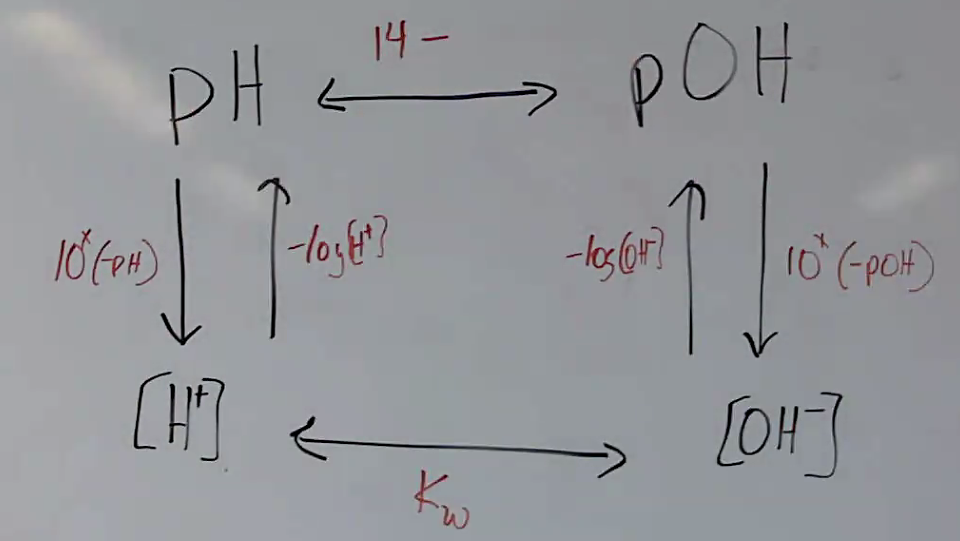
\includegraphics[width=.7\textwidth]{Figures/pHflow.png}
      \caption{pH Flow Chart}
      \label{fig:1}
    \end{figure}
  \end{center}

\item Strong Acid $-$ Completely dissociates (\ce{HCl}, \ce{H2SO4}, \ce{HNO3}, \ce{HClO4}, \ce{HBr}, and \ce{HI})

\item Strong Base $-$ Completely dissociates, hydroxides of columns I and II

\item Weak Acids and Bases $-$ Set up equilibriums

\item $k_w=k_a \cdot k_b$ ($k_w=1\cdot10^{-14}$)

\item p$k_a$=$-\log_{10}(k_a)$, higher $k_a$ means stronger acid

\item Percent Ionization = $\frac{[\ce{H+}]}{[\ce{H}_{\text{acid}}]}\cdot 100\%$ tells how much acid has broken up

\item Polyprotic acids $-$ Give up more than one $[\ce{H+}]$ (ex. \ce{H2C2O4})

\item Stronger Acid, $[\ce{H+}]\uparrow$, $p\ce{H}\downarrow$, $k_a\downarrow$, p$k_a\uparrow$

\item $k_w$ is different at different temperatures

\end{itemize}

\end{document}

